\section{Concept}
%TODO: Paste concept and make it awesome


\subsection{First Idea}


The first idea about this application came to us because our team member Jakub is using an online note taking tool  (in this case apple notes) to keep track of his weekly schedule. Using this note tool to organize the schedule requires more work than necessary. Furthermore it can become a little bit unclear to navigate around the different days and tasks for the week. As we conducted research we were not able to find any application that supports the functionality we would like, meaning an application that has functionality that could be described as some kind of mix between a calendar app and a simple todo list. Our goal is to create an application that lets you plan your task for the next 7 days but not any further. In order to have the schedule available at all times and all devices we decided to create a responsive web application that can run on any device with a modern browser, including desktop computers, smartphones and tablets. User registration and authentication permits for anyone to use this app for his personal schedule planning. The image below shows an example of how our team member Jakub used his note taking app to create his weekly schedule. There is a section for each day of the week as well as another section “stack” for unassigned tasks.   

	\begin{figure}[H] 
		\centering 
		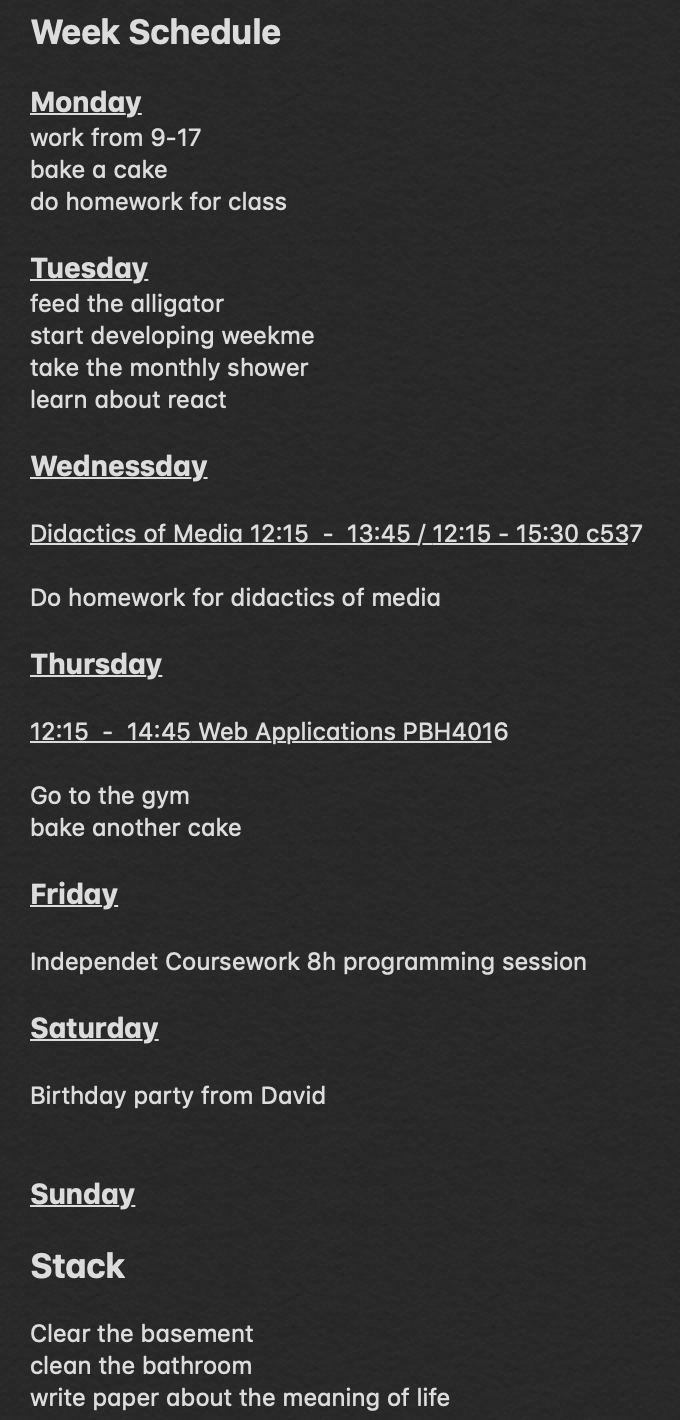
\includegraphics[height=12.2cm]{figures/idea}     
		\caption{Schedule inside Note Taking App}     
	\end{figure}  

\cleardoublepage 

\subsection{First Draft}  
	
The image below demonstrates our first draft of our WeekMe application. The days monday to friday each get their own separate space as well as the stack where unassigned task are collected. Each task is represented by a rectangle. Rectangles can be edited, moved around to another day or to the stack or deleted. For our first prototype we decided to use a framework called Gridstack.js. This framework provides functionality for creating flexible and automatically resizable grids that adapt to its contents. The different task within the grid can be moved around by using drag\&drop. To make sure user always are aware which day of the week we currently have we decided to highlight the current day in a different color. In order to not lose any unfinished tasks we decided to move them back to the stack once their due day has passed. Our top priority was to create a simple and clear user interface and include only the very least functionality that is needed to plan ahead one week and not more.   
 
 	\begin{figure}[H] 
		\centering 
		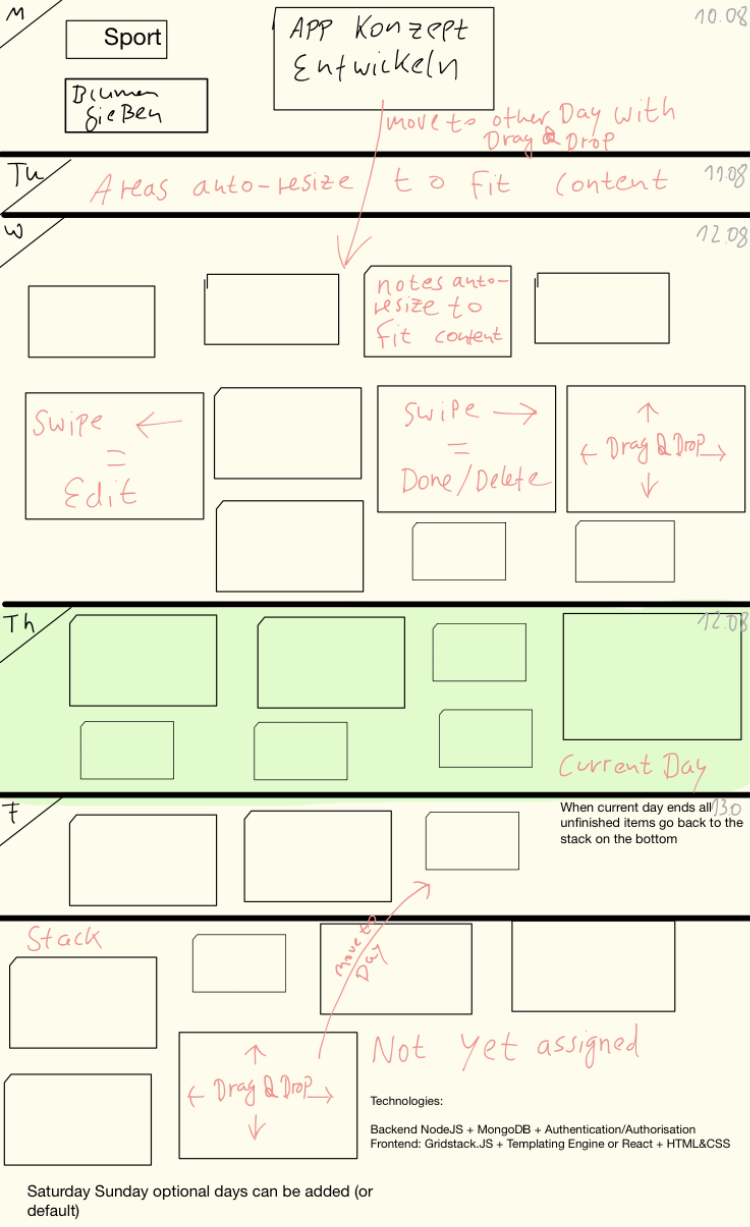
\includegraphics[height=14.2cm]{figures/firstdraft}    
		\caption{First Draft}     
	\end{figure}  







